%\externaldocument[-f]{c2_foundations}
%\externaldocument[-f]{c3_simulation_experiments}
\chapter{Results}
\label{chap:4}
The experimental results are presented in this chapter. First, the parameters for the variables introduced in \cref{chap:3} are given. Then a sample of simulated trajectories are shown as an example. Finally, the inference results are presented.

\section{Configurations}
\label{sec:config}
The configurations given below are used for the results presented in the following sections, if not specified otherwise.
\begin{itemize}
	\item Gamma priors for parent dynamics such that $ \textbf{Q}_{i} \sim \mathrm{Gam}(\symbf{\alpha}^i, \symbf{\beta}^i)$ for $i \in \left\lbrace 1,2\right\rbrace $, and $ \symbf{\alpha} = [\alpha_0, \alpha_1] $ and $ \symbf{\beta} = [\beta_0, \beta_1] $
	\begin{align}
	\symbf{\alpha}^1 = [5,10] &\quad \symbf{\beta}^1 = [5,20] \\
	\symbf{\alpha}^2 = [10,10] &\quad \symbf{\beta}^2 = [10,5]
	\label{eq:gamma_params}
	\end{align}
	\item Transition intensity matrices of $ X_1 $ and $ X_2 $ sampled from priors given above
	\begin{align}
	\textbf{Q}_1 &= 
	\begin{bmatrix}
	-1.117 & 1.117 \\
	0.836 &  -0.836
	\end{bmatrix} \\
	\textbf{Q}_2 &= 
	\begin{bmatrix}
	-1.1 & 1.1 \\
	2.445 &  -2.445
	\end{bmatrix}
	\end{align}
	\item Length of trajectories $ T = 5\text{s} $
	\item State space, $ \rchi_{P} = \rchi_1 \times \rchi_2 = \left\lbrace (x_1, x_2)\right\rbrace_{x_1\in \rchi_1, x_2\in \rchi_2} = \left\lbrace (0, 0), (0, 1), (1, 0),(1, 1)\right\rbrace $
	\item Observation space, $ \mathcal{Y} = \left\lbrace 0, 1, 2 \right\rbrace $
	\item Action space, $ \textit{A} = \left\lbrace a_{0}, a_{1} \right\rbrace = \left\lbrace 0, 1\right\rbrace $
	\item The set of transition intensity matrices of $ X_3 $
	\begin{align}
	\textbf{\textit{Q}}_3 = \left\lbrace \textbf{Q}_{3\mid a_{0}}, \textbf{Q}_{3\mid a_{1}} \right\rbrace = \left\lbrace 
	\begin{bmatrix}
	-0.5 & 0.5 \\
	2 &  -2
	\end{bmatrix}, 
	\begin{bmatrix}
	-3 & 3 \\
	0.02 &  -0.02
	\end{bmatrix} 
	\right\rbrace 
	\end{align}
	\item Number of particles, $ N = 200 $
	\item Weights of the policy introduced in \autoref{eq:policy}, $ \textbf{w} = [0.02, 0.833, 0.778, 0.87] $
	\item Observation model
	$\psi_{\text{true}} =
	\begin{bmatrix}
		1 & 0 & 0 \\
		0 & 1 & 0 \\
		0 & 1 & 0 \\
		0 & 0 & 1
	\end{bmatrix}$
%	\item Simulation parameters $  \theta_sim = \left\lbrace  \textbf{Q}_{1}, \textbf{Q}_{2}, \textit{\textbf{Q}}_3, \textbf{w}, \psi_{\text{true}} \right\rbrace $
\end{itemize}
%In the following, $ \psi_{\text{true}} $ denotes the observation model which is used for data generation in the given results.

\section{Simulation}
\label{sec:simulation}
The synthetic dataset is generated utilising \cref{alg:sampling}. K trajectories in time interval $ [0, T] $ are denoted by $ \xi_T = \left\lbrace S^{[0,T], 1}, S^{[0,T], 2}, ..., S^{[0,T], K} \right\rbrace  $, where $ S^{[0,T],k} = \left\lbrace X_1^{[0,T],k} , X_2^{[0,T],k}, X_3^{[0,T],k}\right\rbrace $ denotes a single trajectory for all nodes. It is noteworthy that the initial states are drawn from disrete uniform distribution.
\begin{equation}
X_i(0) \sim \mathcal{U} \left\lbrace 0, 1\right\rbrace  \text{ for } i \in \left\lbrace 1,2,3\right\rbrace 
\end{equation}
\autoref{fig:parent_traj}(a)-(b) shows an example of parent trajectories. In \autoref{fig:parent_traj}(c), the resulting trajectory of the joint parent process $ X_P $ is illustrated. As mentioned in \cref{sec:exp_ctbn_model}, this joint process over the parent nodes provides a compact representation. 
\begin{figure}[H]
	\begin{center}
		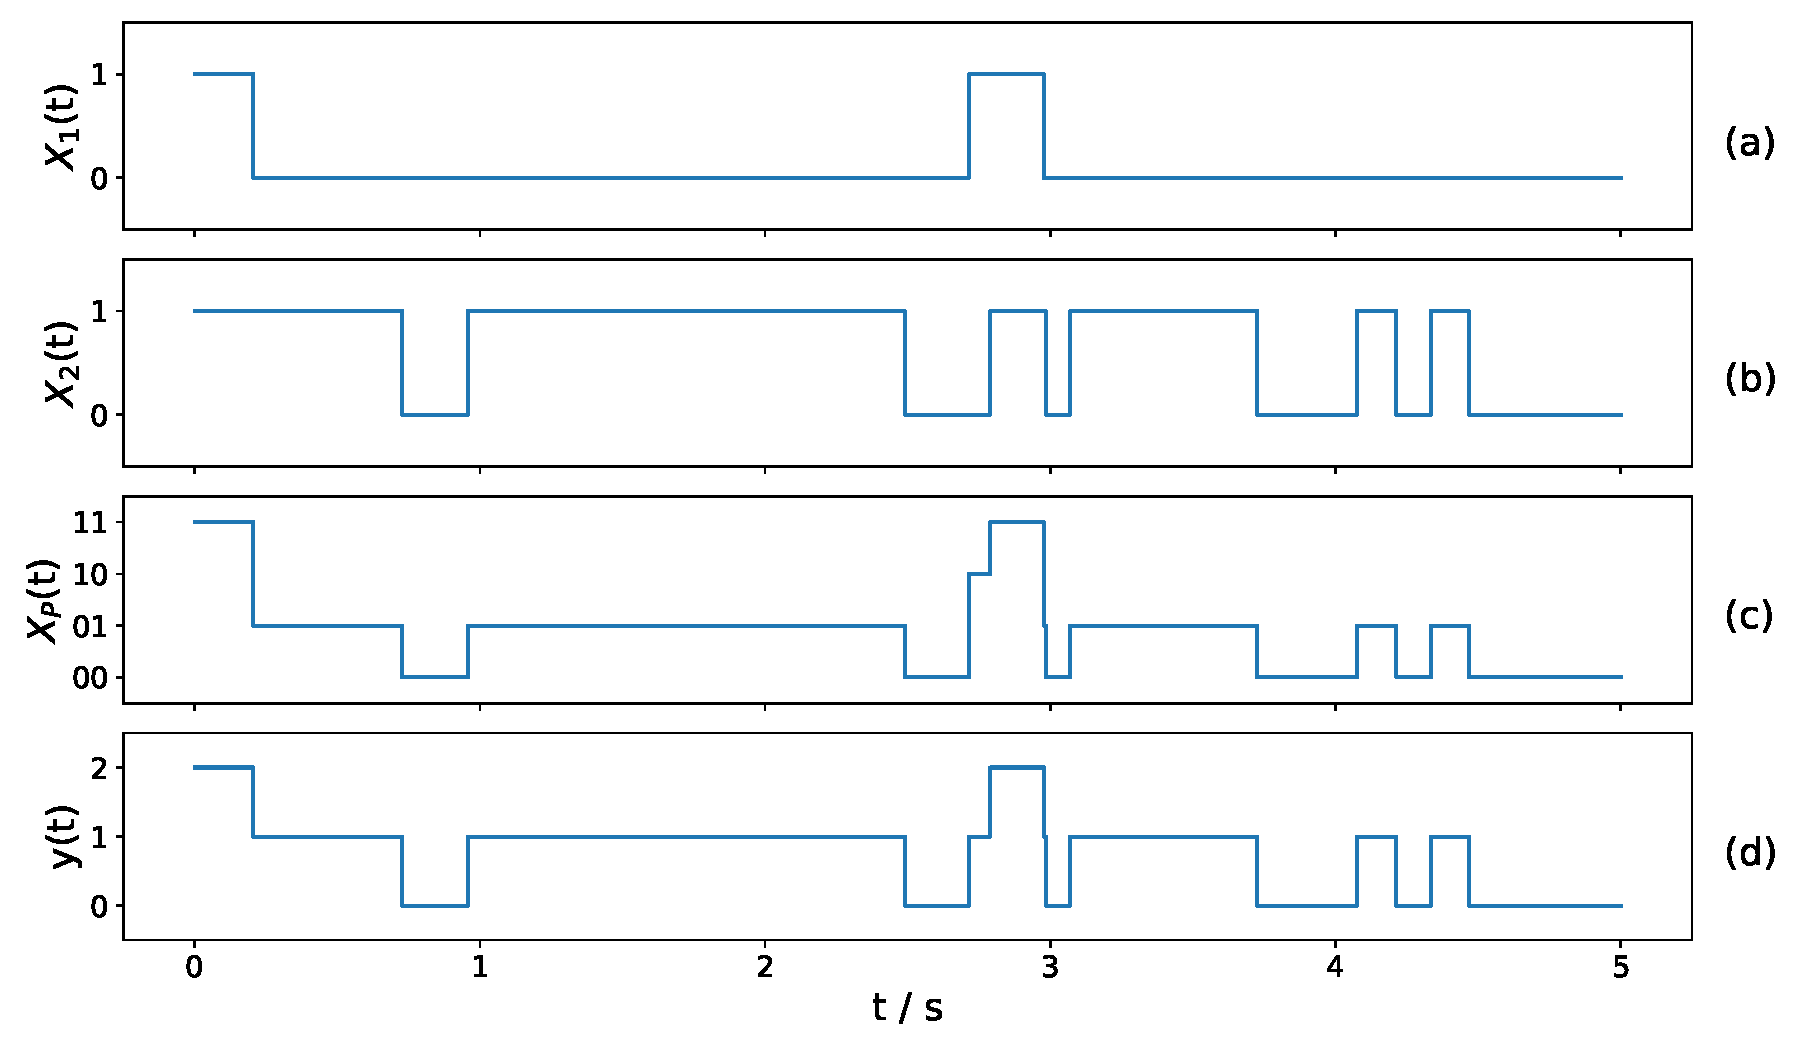
\includegraphics[width=.90\textwidth]{figures/sim_example/parent_traj}
		\caption[Parent trajectories and observation]{A sample of parent trajectories and observation. (a)-(b) A sample trajectory of parent nodes $ X_1 $ and $ X_2 $ of length $ T=5\text{s} $, (c) The trajectory of the joint parent process $ X_P $, (d) The observation trajectory resulting from $ X_P $ given in (c) and $ \psi_{\text{true}} $ given in \cref{sec:config}.}
		\label{fig:parent_traj}
	\end{center}
\end{figure}
In \autoref{fig:parent_traj}(c), the states of $ X_P $ taking values in $ \rchi_P = \rchi_1 \times \rchi_2 $ is preferred to be represented as a combination of the parent states for readibility, so that $ \rchi_P = \left\lbrace 00, 01, 10, 11\right\rbrace  $, where $ x_P \in \rchi_P $ simply corresponds to $ x_1x_2,\ x_1\in \rchi_1,\  x_2\in \rchi_2 $. \autoref{fig:parent_traj}(d) shows the observation trajectory resulting from $ X_P(t) $ and the observation model $ \psi_{true} $ given in \cref{sec:config}. \\
\autoref{fig:belief_traj} illustrates the belief state trajectory given the observations in \autoref{fig:parent_traj}(d). For the reference, the belief state update using particle filter and exact update is given together. As can be seen from the figures, the exact update is well approximated by the particle filter.
\begin{figure}[H]
	\begin{center}
		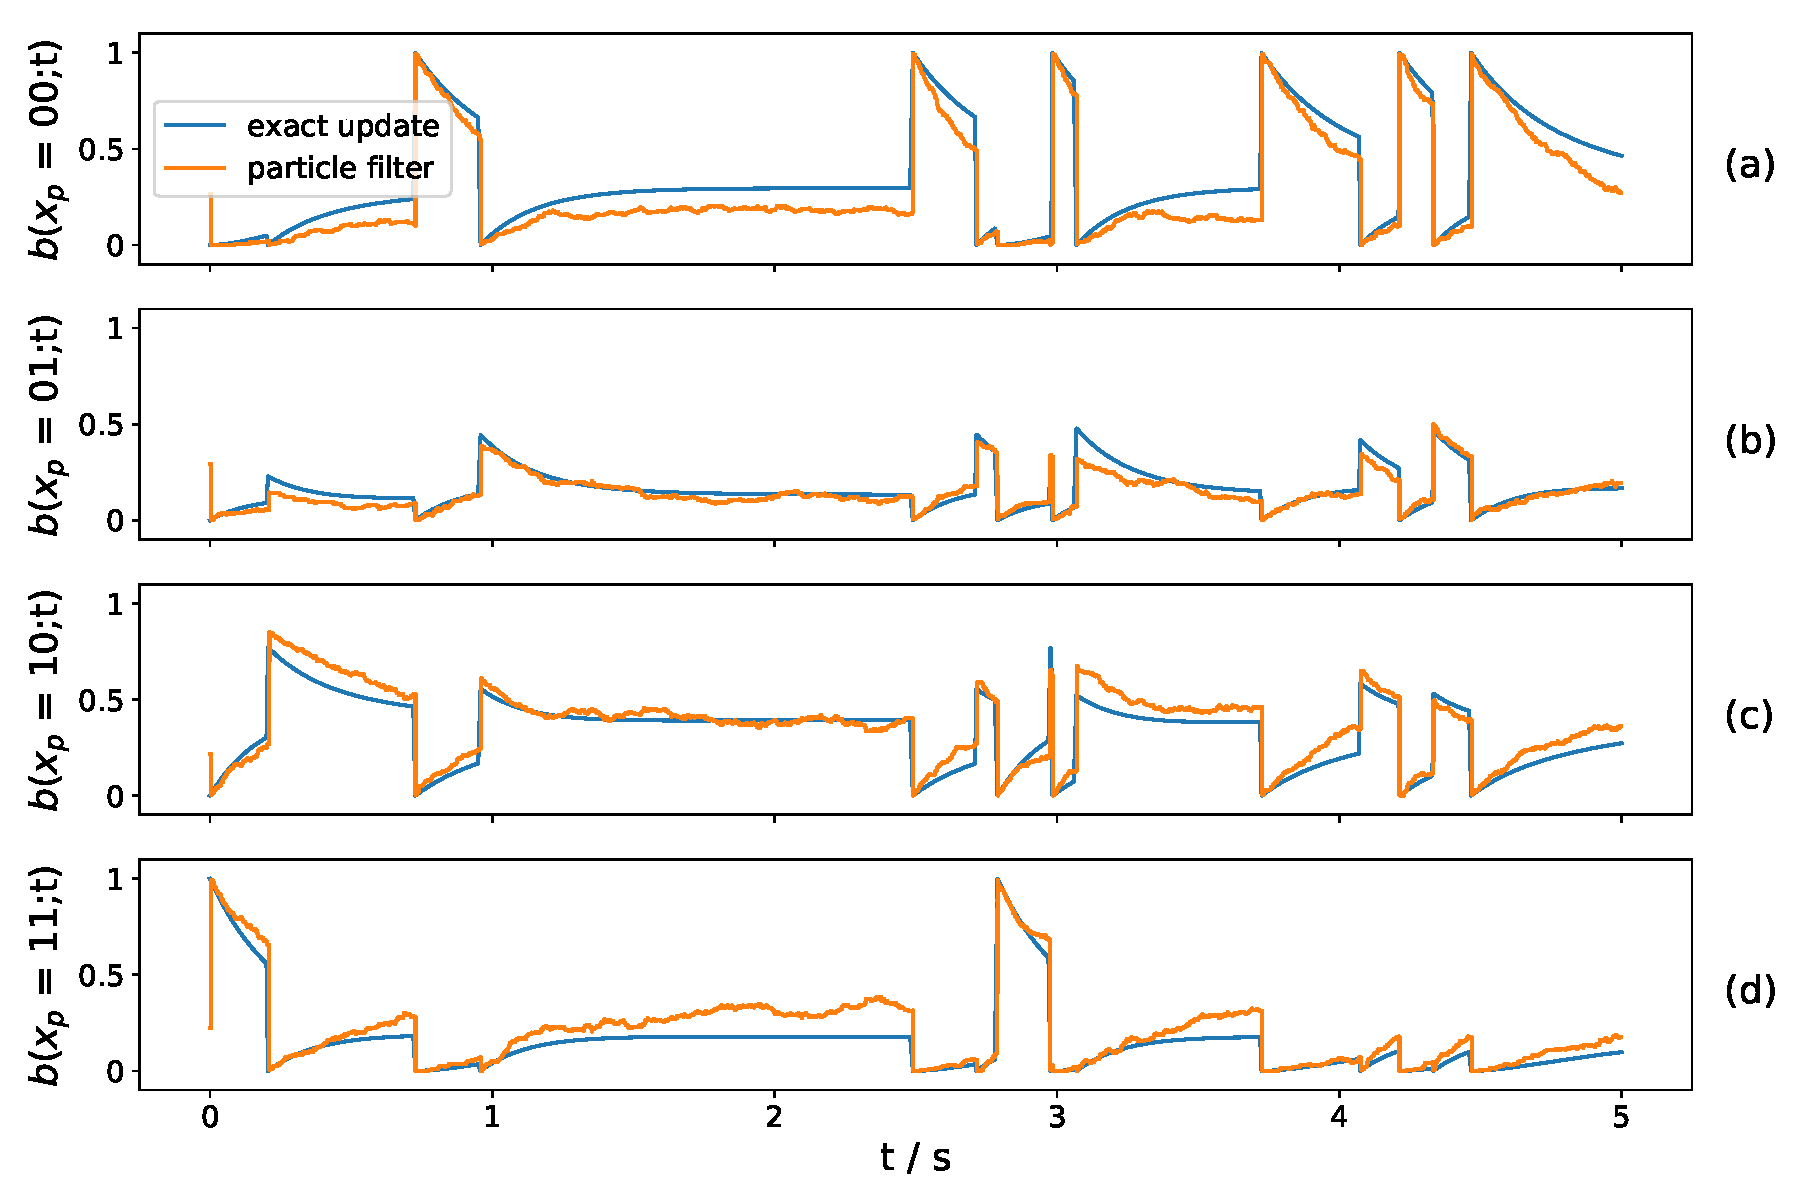
\includegraphics[width=.9\textwidth]{figures/sim_example/belief_traj}
		\caption[Belief state trajectories]{Belief state trajectories corresponding to the observations given in \autoref{fig:parent_traj}(d), comparing exact update method and particle filtering.}
		\label{fig:belief_traj}
	\end{center}
\end{figure}
Finally, the resulting $ Q_3 $ and the trajectory of agent are given in \autoref{fig:q_traj}. The $ Q_3 $ trajectory shown in \autoref{fig:q_traj}(b), are derived from the belief state update by particle filter which is given in \autoref{fig:q_traj}(a) using \autoref{eq:policy} and \autoref{eq:Q_3_traj}.
\begin{figure}[H]
	\begin{center}
		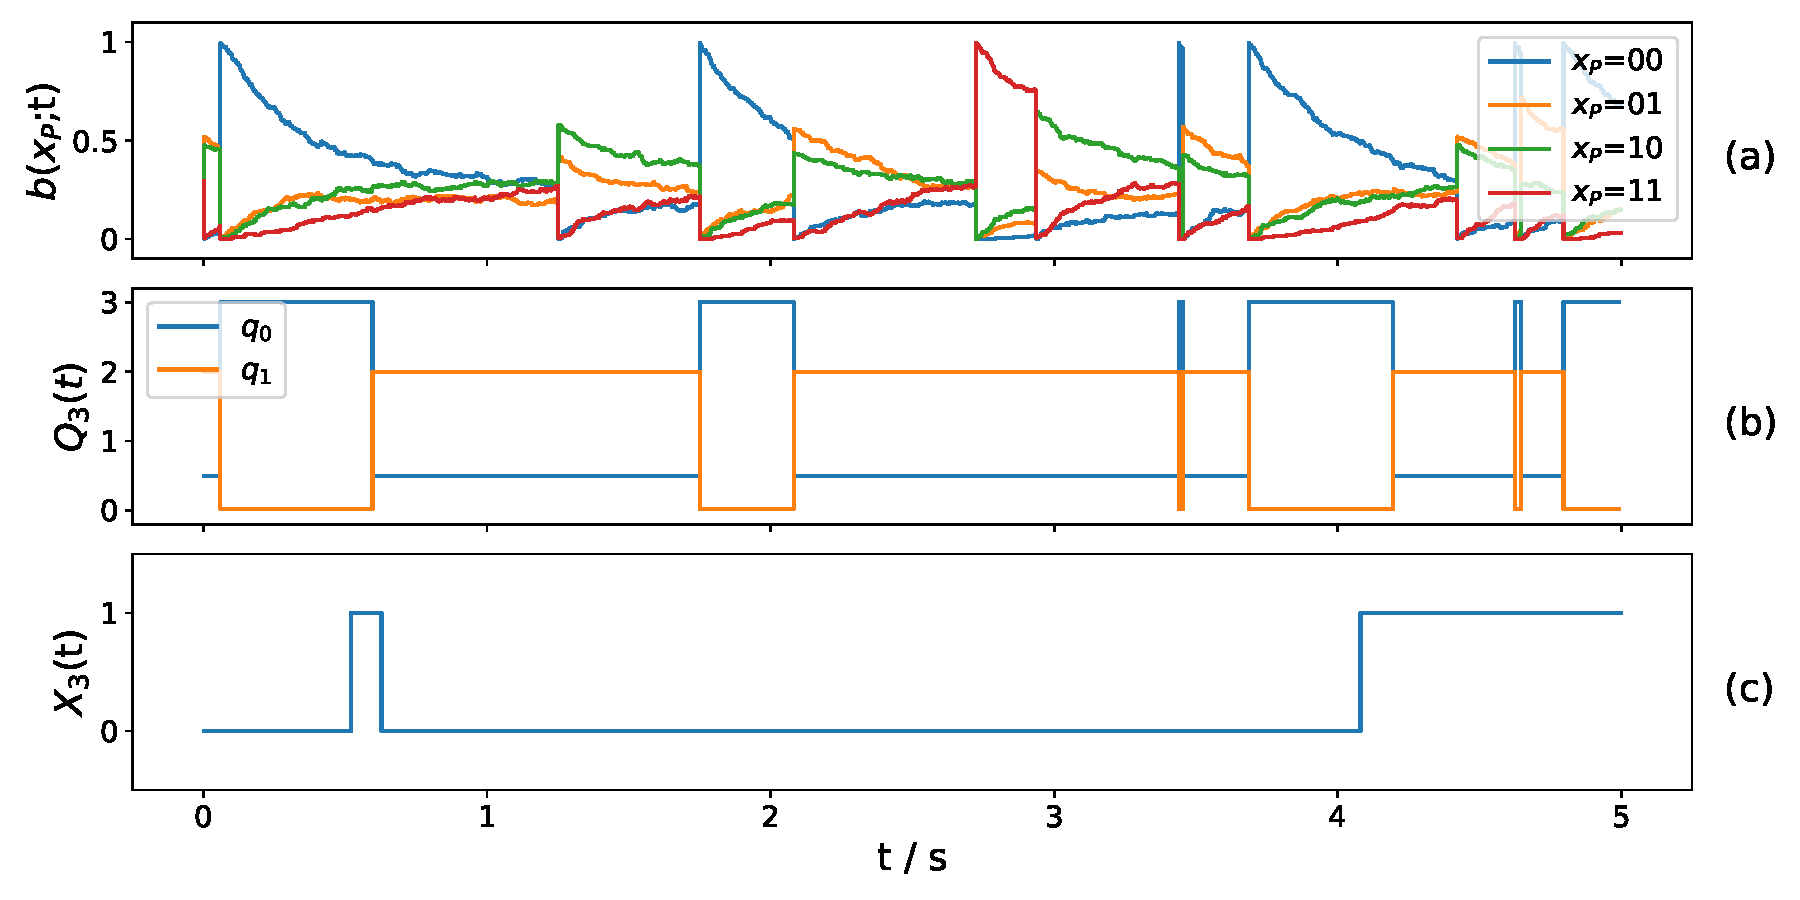
\includegraphics[width=.9\textwidth]{figures/sim_example/q_traj}
		\caption[$ Q_3 $ and $ X_3 $ trajectories]{Belief state updated by particle filter and the resulting $ Q_3 $ and $ X_3 $ trajectories.}
		\label{fig:q_traj}
	\end{center}
\end{figure}
As mentioned in \cref{par:bs_partFilt}, the degeneration of the particle filter in case of an unlikely changes in observation, i.e. unanticipated transitions of parent nodes, is handled by by assigning uniform probabilities to the particles. It effectively corresponds to ignoring the rapid changes of the observation, which may cause diverging from the exact update, however, it is recovered with the next observation. \autoref{fig:deg_partFilter} provides an example of the sitution. The rapid change in question that caused particle filter method to diverge from exact update method is highlighted in \autoref{fig:deg_partFilter}(a). The particles fail to simulate this observation, and due to uniformization, the transition from 2 to 1 is ignored by the particle filter method. The divergence can be observed in \autoref{fig:deg_partFilter}(d)-(e) clearly.
\begin{figure}[H]
	\begin{center}
		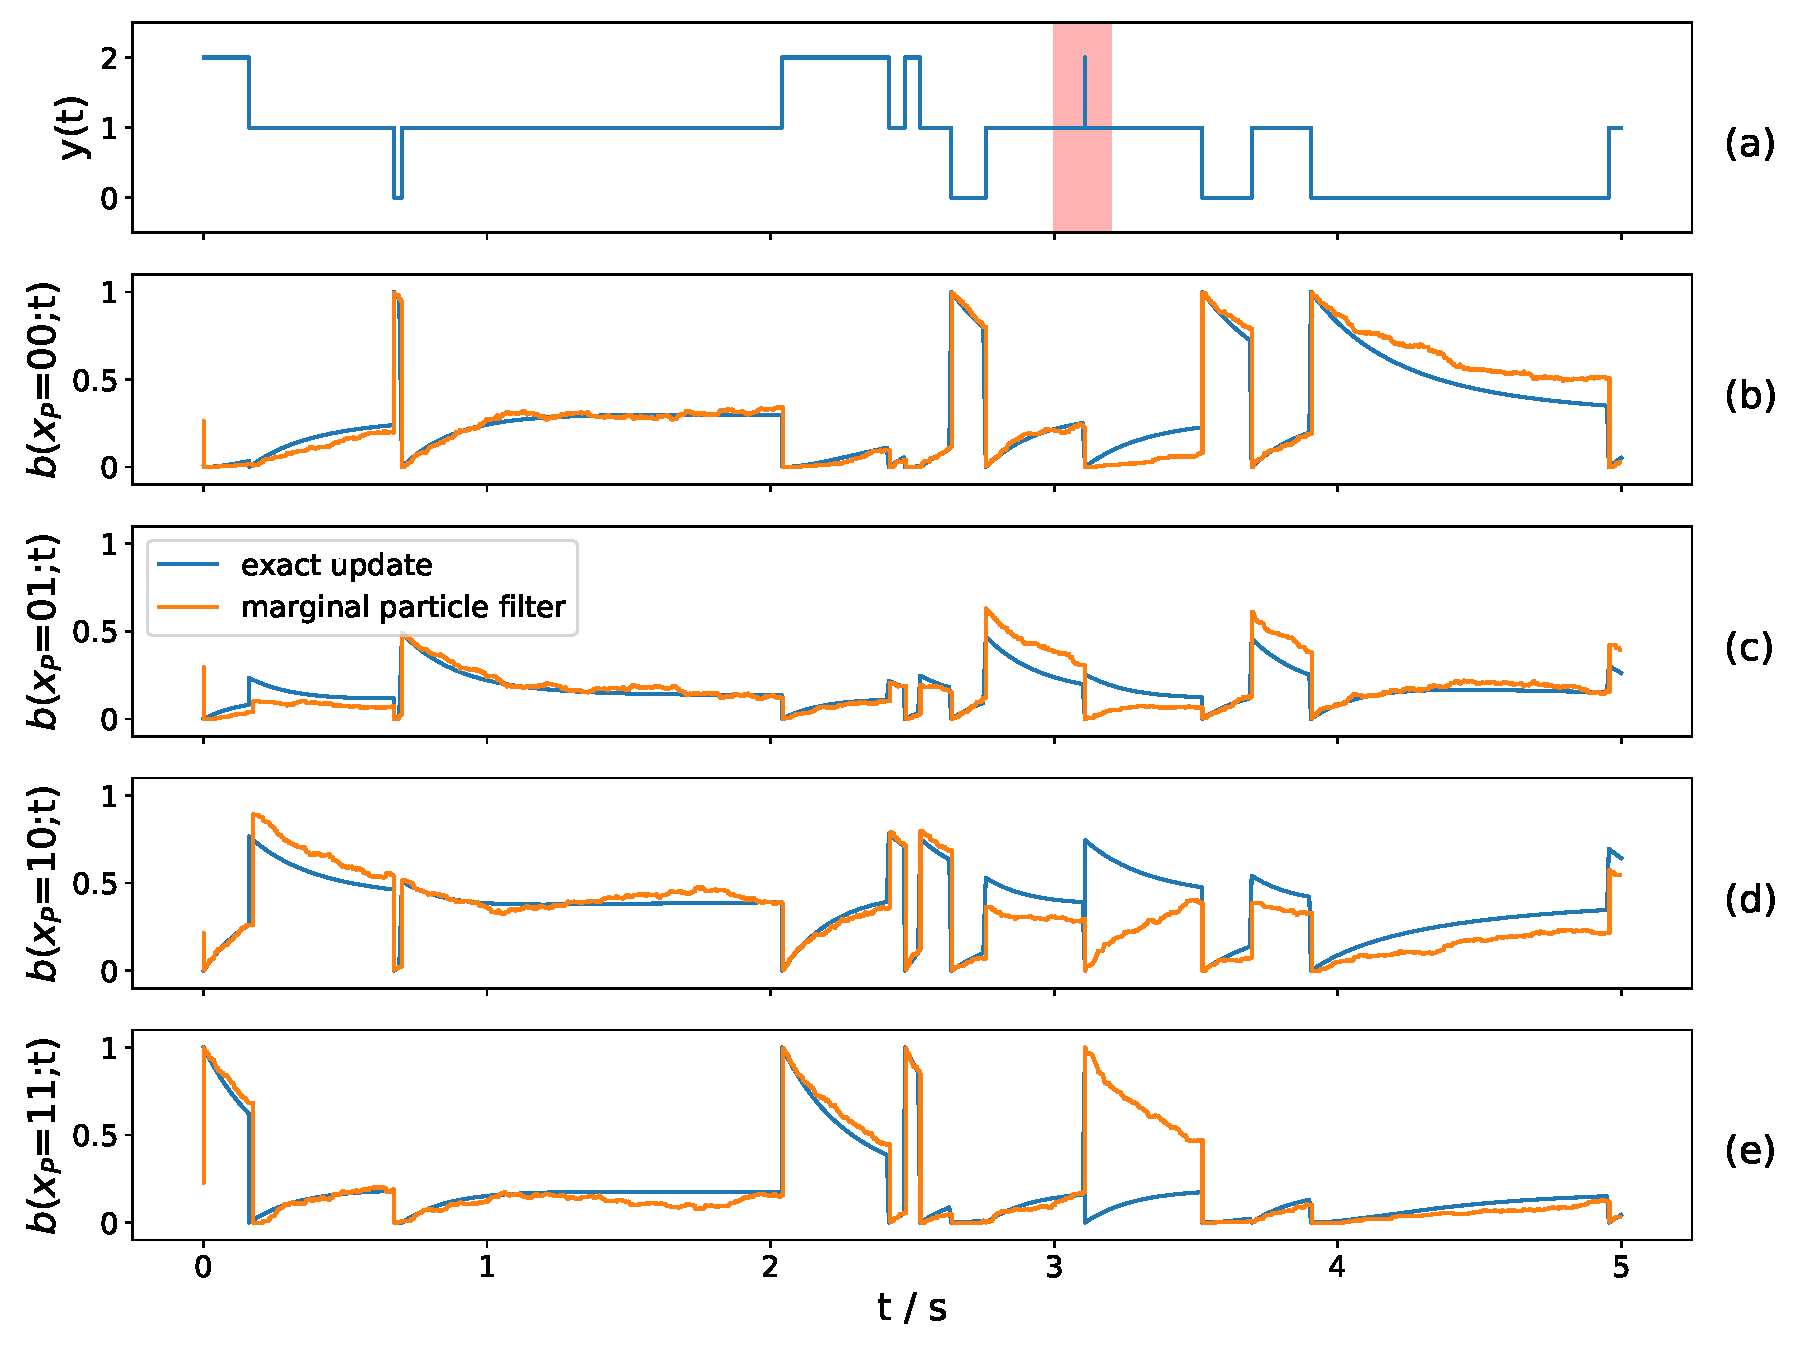
\includegraphics[width=.90\textwidth]{figures/degenerate_pf/belief_traj}
		\caption[Degenerate particle filter]{A sample with degenerate particle filter. The unlikely observation which has caused the degeneration is highlighted in (a). It can be seen in (d) and (e) that this observation causes particle filter approximation to diverge from exact update results but it is recovered with the next observation.}
		\label{fig:deg_partFilter}
	\end{center}
\end{figure}

\section{Inference of Observation Model}
We considered the problem of inferring the observation model as a classification problem. As a measure of the performance of the classifier, we utilised area under the Reciever-Operator-Characteristic curve (AUROC) and Presition-Recall curve (AUPR). 
\subsection{Equivalence Classes}
\label{sec:eq_classes}
As mentioned in \cref{sec:inf_setup}, the deterministic nature of the observation model results in a number of possible observation models. The setting described in \cref{chap:3} with configurations given in \cref{sec:config} leads to 81 obsevation models. However, with this experimental setup and the methods, it is only possible to distinguish these observation models into 10 different classes. Due to this equivalence, the inference problem is considered only for 10 observation models, each one representing one class. The reasons of this phenomena are discussed in detail in \cref{ap:eq_classes}, together with the observation models considered in the inference problem. The set of observation model that can be classified is denoted as $ \symbf{\psi} $ in the following. \\
\autoref{fig:llh_exactUpdate_81model} illustrates the equivalence of observation models clearly. The plot depicts the results of an experiment with 200 samples, $ |\xi_T| = 200 $, generated using the observation model $ \psi_{\text{true}} $ given in \cref{sec:config}, and the average log-likelihood of samples computed for all possible observation models. Here, the belief state is updated using exact method as described in \cref{par:bs_exact}, in order to depict the exact equivalence within one class. As can be seen, the results show the separation of the set of observation models into 10 distinct classes. The legend is removed to avoid clutter.
\begin{figure}[H]
	\begin{center}
		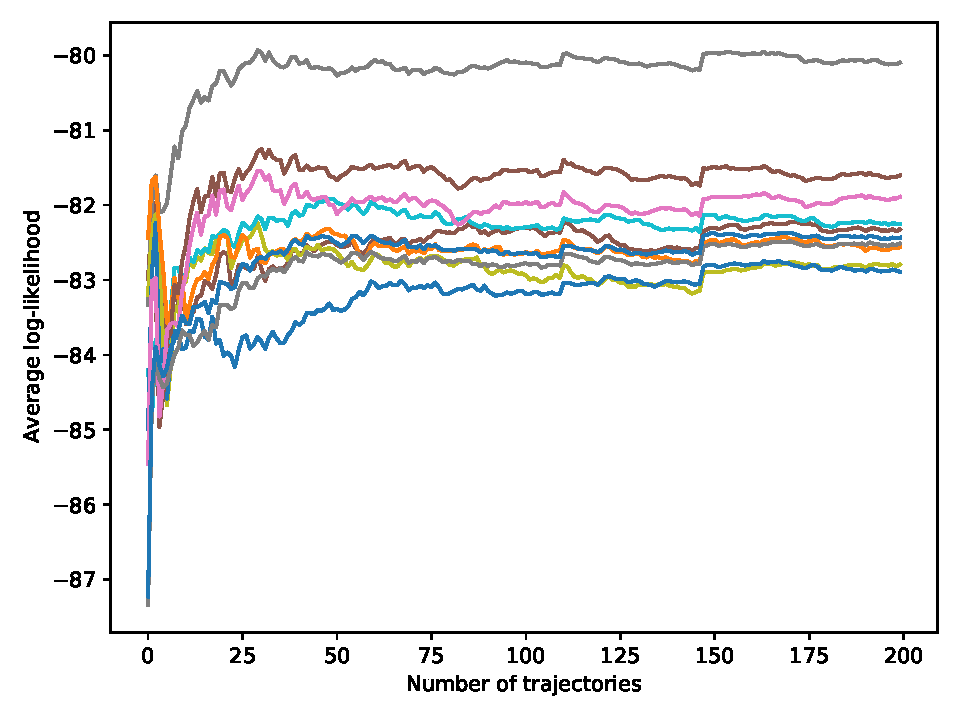
\includegraphics[width=.8\textwidth]{figures/equivalence_classes/llh_exactUpdate_81model}
		\caption[Equivalence classes in the case of exact belief update]{Average log-likelihood $ \log p(S^{[0,T]} \mid \theta) $ over samples generated using exact belief state update, depicting the equivalence classes in the set of observation models.}
		\label{fig:llh_exactUpdate_81model}
	\end{center}
\end{figure}
In order to show the validity of the equivalence in the case of particle filter, the average log-likelihoods of 200 samples given two observation models in the same class are illustrated in \autoref{fig:llh_particleFilter_sameclass}. The samples are generated with $ \psi_{\text{true}} = \psi_{0} $, and the rest of the observation models here fall in the same equivalence class as $ \psi_0 $. As can be seen from the graph, the observation models lead to so similar results to each other that they are assumed to be identical. 
\begin{figure}[H]
	\begin{center}
		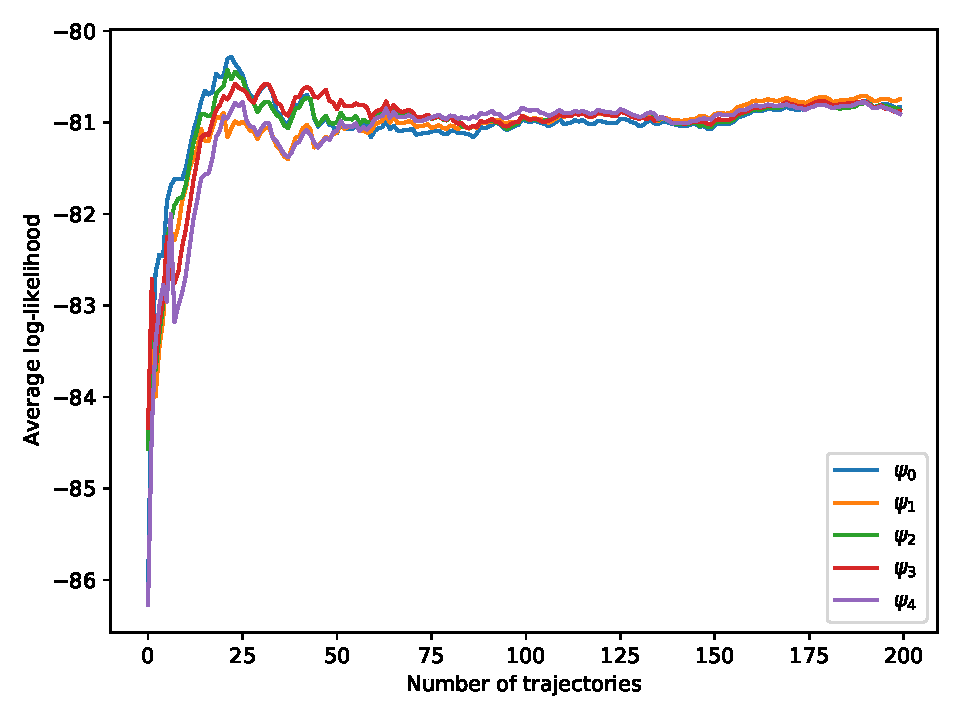
\includegraphics[width=.8\textwidth]{figures/equivalence_classes/llh_particleFilter_sameclass}
		\caption[An equivalence class in the case of particle filtering]{Average log-likelihood $ \log p(S^{[0,T]} \mid \theta) $ over samples generated using particle filtering, where $ \psi_1 $ and $ \psi_2 $ belongs in the same class.}
		\label{fig:llh_particleFilter_sameclass}
	\end{center}
\end{figure} 
\subsection{Learning Observation Model}
\autoref{fig:llh_exact} illustrates the average log-likelihood over 100 samples given the observation models. The samples are generated with $ \psi_{true} = \psi_0 $ given in \cref{sec:config}, and exact update method is utilised for belief state update. As can be seen, the curves converge quicly and the true model is well separated from others. Consequently, the maximum likelihood estimation by \autoref{eq:max_llh_est} leads to the correct result. \\
A similar experiment is documented in \autoref{fig:llh_particle}, where exact update method is replaced by particle filtering. $ \psi_0 $ denotes the observation model that has generated the dataset, and it is correctly estimated as the true model. The jump around 50 trajectories can be explained by an encounter with a highly likely parent trajectories.
\begin{figure}[H]
	\begin{center}
		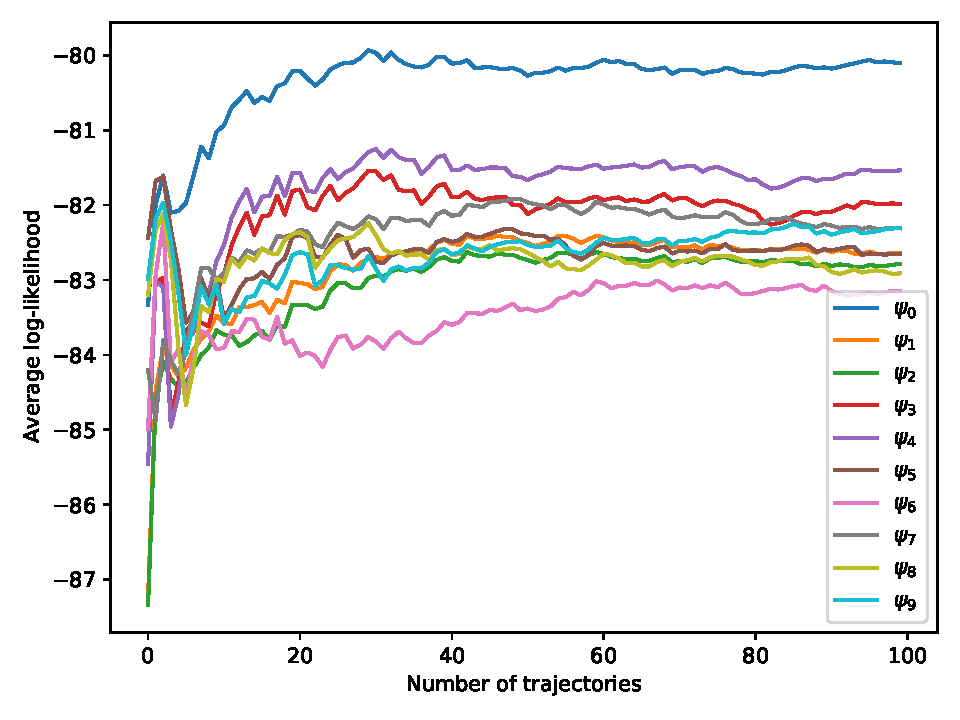
\includegraphics[width=.75\textwidth]{figures/roc_analysis/roc_exactUpdate/llh_exactUpdate_psi_0}
		\caption[Average log-likelihood in the case of exact belief update]{Average log-likelihood $ \log p(S^{[0,T]} \mid \theta) $ with $ \psi_i \in \symbf{\psi} $ over samples generated using exact belief state update}
		\label{fig:llh_exact}
	\end{center}
\end{figure}
\begin{figure}[H]
	\begin{center}
		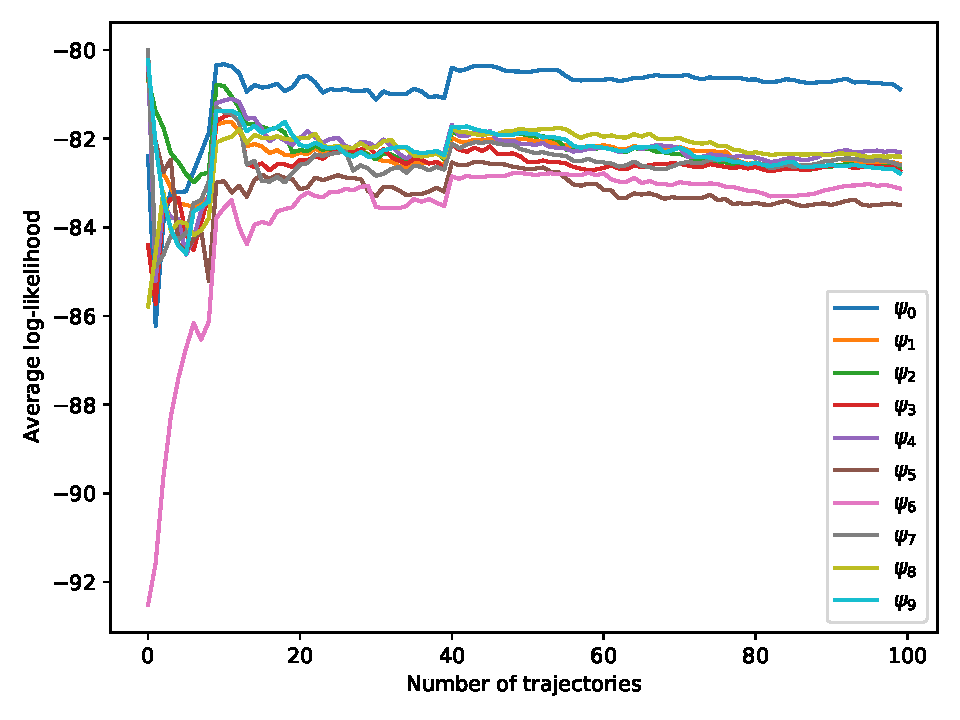
\includegraphics[width=.75\textwidth]{figures/roc_analysis/roc_particleFilter/llh_particleFilter_psi_0}
		\caption[Average log-likelihood in the case of particle filtering]{Average log-likelihood $ \log p(S^{[0,T]} \mid \theta) $ with $ \psi_i \in \symbf{\psi} $ over samples generated using particle filtering}
		\label{fig:llh_particle}
	\end{center}
\end{figure}
We approach the inference problem as classification between the observation models $ \psi \in \symbf{\psi} $ given in \cref{ap:obs_set_exp}. We consider the estimated likelihood values of each sample given an observation model as the score of the sample belonging to the corresponding class. Since this setting represents a multi-class classification problem, the
performance metrics AUROC and AUPR are calculated as one-vs-rest. \\ %performance metric AUROC is calculated as one-vs-rest. \\ %
Consider a binary classification problem. True positives (TP) are the samples predicted as 1 correctly, and false positives (FP) are the samples predicted as 1 while the true label was 0. True negatives (TN) are the samples predicted as 0 correctly, and false negatives (FN) are the samples with true label 1, but predicted 0. True positive rate (TPR), also called \textit{recall} (R) or \textit{sensitivity}, is the ratio of TPs over the number of samples which are labelled as 1. False positive rate (FPR) is the ratio of FPs over the number of samples labelled as 0. The precision (P) is the ratio of TPs over the number of all the samples predicted as 1.
\begin{align}
\text{TPR} = \text{R} &= \frac{\text{TP}}{\text{TP} + \text{FN}} \\
\text{FPR} &= \frac{\text{FP}}{\text{TN} + \text{FP}} \\
\text{P} &= \frac{\text{TP}}{\text{TP} + \text{FP}}
\end{align}
Receiver Operating Characteristics (ROC) curve illustrates the tradeoff between true positives and false positives, over different values of threshold for classification \cite{Robinson2008}. The area under ROC curve (AUROC) is a performance metric that shows how well the classifier can distinguish the classes. Higher AUROC metric indicates better performance, taking values in the interval [0,1]. Precision-Recall (PR) curve illustrates the relation between precision and recall, providing a metric to quantify how many of the predictions were correct \cite{Boyd2013}.\\
We provided the classifier with increasing number of samples for inference. This is achieved through bootstrapping a given number of trajectories, and using the mean likelihood over the bootrap batch as a new sample. The following AUROC plots shows the results over 50 trajectory generated using each obervation model as the true model. According to this, in our dataset, we have 500 trajectories, 50 from each class labelled through a vector with 10 entries, having only 1 for the true observation model and 0 for the rest. When number of trajectories is 1, each sample in the dataset considered individually. When number of trajectories is 2, within each class, 50 sample batches of size 2 are bootstrapped such that none of the batches consist of the same samples. By doing so, we keep the sample size at 50 per each class, regardless of the batch size. \\
\autoref{fig:AUROC_class0} shows the AUROC results over 10 runs, comparing the state estimator using exact update and particle filtering. We plotted the median AUROC as a line and 25-75\% percentile as the shaded area. \autoref{fig:AUPR_class0} illustrates the AUPR in the same manner. As expected given the unbiased classifier, both metrics approach to 1 as the number of samples increases. Due to the stochasticity introduced by the particle filtering as the state estimator, the results obtained with this method show slightly lower performance. 
%As expected given the unbiased classifier, this metric approaches to 1 as the number of samples increases. Due to the stochasticity introduced by the particle filtering as the state estimator, the results obtained with this method show slightly lower performance. 
\begin{figure}[H]
	\begin{center}
		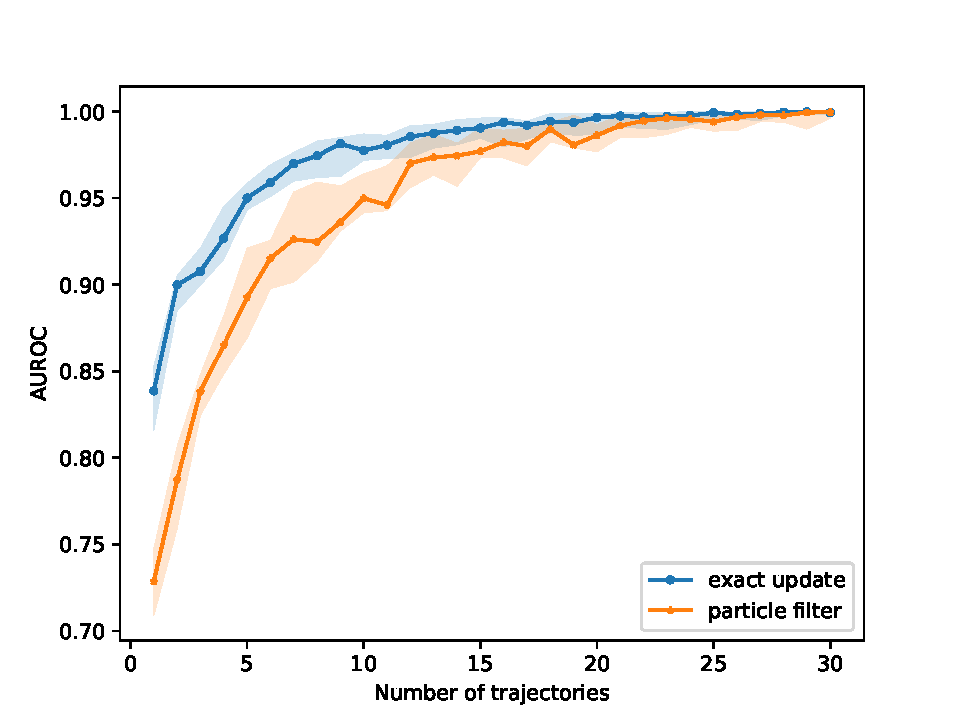
\includegraphics[width=.75\textwidth]{figures/roc_analysis/AUROC_perc_0}
		\caption[AUROC results over increasing number of samples]{AUROC results over increasing number of samples for $ \psi_0 $-vs-rest. We plotted the median with line and the 25-75\% percentile with the shaded area over 10 runs.}
		\label{fig:AUROC_class0}
	\end{center}
\end{figure}
\begin{figure}[H]
	\begin{center}
		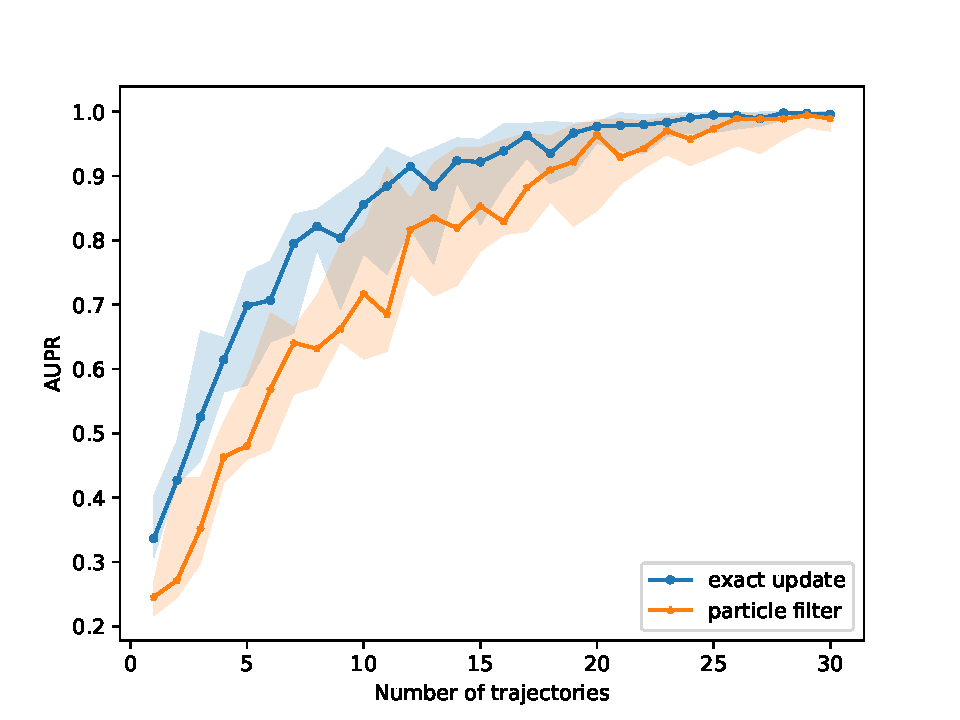
\includegraphics[width=.75\textwidth]{figures/roc_analysis/AUPR_perc_0}
		\caption[AUPR results over increasing number of samples]{AUPR results over increasing number of samples for $ \psi_0 $-vs-rest. We plotted the median with line and the 25-75\% percentile with the shaded area over 10 runs.}
		\label{fig:AUPR_class0}
	\end{center}
\end{figure}
\subsection{Robustness Test under Channel Noise}